\documentclass[a4paper, 12pt]{report}
\usepackage{template_tugas_akhir_fte}

\begin{document}
\onehalfspacing
\newacronym{ieee}{IEEE}{Institute of Electrical and Electronics Engineers}
\newacronym{ta}{TA}{Tugas Akhir}
\newacronym{kbbi}{KBBI}{Kamus Besar Bahasa Indonesia}
\newacronym{iot}{IoT}{Internet of Things}

\begin{titlepage}
   \begin{center}

   % ==================================================
   % Judul Tugas Akhir dalam Bahasa Indonesia
   % Gunakan huruf kapital pada setiap kata penting
   % ==================================================
   \large\MakeUppercase{\textbf{Judul dalam Bahasa Indonesia}}\\
   % Contoh:
   % Sistem Deteksi Burung Berbasis TinyML untuk Monitoring Keanekaragaman Hayati

   \vspace{2em}

   % ==================================================
   % Judul Tugas Akhir dalam Bahasa Inggris
   % Terjemahan resmi dari judul Bahasa Indonesia
   % ==================================================
   \large\MakeUppercase{\textit{Title in English}}\\
   % Example:
   % TinyML-Based Bird Detection System for Biodiversity Monitoring

   \vspace{2em}

   % Jenis dokumen
   \MakeUppercase{\textbf{Tugas Akhir}}\\

   % Keterangan pengajuan tugas akhir
   \normalsize Diajukan sebagai syarat mata kuliah Tugas Akhir\\

   % ==================================================
   % Nama program studi
   % Sesuaikan dengan program studi mahasiswa
   % ==================================================
   Program Studi S1 Teknik Fisika \\
   % Contoh:
   % Program Studi S1 Teknik Elektro
   % Program Studi S1 Teknik Telekomunikasi

   \vspace{2em}

   Disusun oleh:\\

   % ==================================================
   % Nama lengkap mahasiswa
   % Ditulis sesuai data akademik
   % ==================================================
   \MakeUppercase{\textbf{NAMA PENULIS}}\\
   % Contoh:
   % AHMAD QURTHOBI

   % ==================================================
   % Nomor Induk Mahasiswa (NIM)
   % ==================================================
   \MakeUppercase{\textbf{NIM PENULIS}}\\
   % Contoh:
   % 120220001

   \vfill

   % ==================================================
   % Logo universitas
   % Pastikan file logo tersedia pada folder Gambar
   % ==================================================
   
\includegraphics[width=0.5\textwidth]{Gambar/logoTelU.png}\\

   \vspace{2em}

   % ==================================================
   % Nama fakultas
   % Sesuaikan jika template digunakan oleh fakultas lain
   % ==================================================
   \large \MakeUppercase{\textbf{Fakultas Teknik Elektro}}\\

   % Nama universitas
   \MakeUppercase{\textbf{Universitas Telkom}}\\

   % Kota universitas
   \MakeUppercase{\textbf{Bandung}}\\

   % Tahun penyusunan / tahun sidang
   \textbf{\the\year}
   % Atau dapat diganti manual, misalnya:
   % \textbf{2026}

   \end{center}
\end{titlepage}

\clearpage
\pagenumbering{roman}
\setcounter{page}{2}


% ==================================================
% Judul halaman
% ==================================================
\chapter*{\MakeUppercase{Lembar Pengesahan}}

% Menambahkan Lembar Pengesahan ke Daftar Isi
\addcontentsline{toc}{chapter}{\MakeUppercase{Lembar Pengesahan}}

\begin{center}

% Jenis dokumen
\large\MakeUppercase{\textbf{Tugas Akhir}}

\vspace{2em}

% ==================================================
% Judul Tugas Akhir dalam Bahasa Indonesia
% ==================================================
\large\MakeUppercase{\textbf{Judul dalam Bahasa Indonesia}}\\
% Contoh:
% Sistem Deteksi Burung Berbasis TinyML untuk Monitoring Keanekaragaman Hayati

\vspace{2em}

% ==================================================
% Judul Tugas Akhir dalam Bahasa Inggris
% ==================================================
\large\MakeUppercase{\textbf{\textit{Title in English}}}\\
% Example:
% TinyML-Based Bird Detection System for Biodiversity Monitoring

\vspace{2em}

% Keterangan pengesahan
\normalsize \textbf{Telah disetujui dan disahkan sebagai Buku Tugas Akhir}\\

% ==================================================
% Nama program studi
% ==================================================
\textbf{Program Studi Teknik Fisika}\\
% Contoh:
% Program Studi Teknik Elektro
% Program Studi Teknik Telekomunikasi

% Nama fakultas
\textbf{Fakultas Teknik Elektro}\\

% Nama universitas
\textbf{Universitas Telkom}\\

\vspace{2em}

\textbf{Disusun oleh:}\\

% ==================================================
% Nama lengkap mahasiswa
% ==================================================
\MakeUppercase{\textbf{NAMA PENULIS}}\\
% Contoh:
% AHMAD QURTHOBI

% ==================================================
% Nomor Induk Mahasiswa (NIM)
% ==================================================
\MakeUppercase{\textbf{NIM PENULIS}}\\
% Contoh:
% 120220001

\vfill

% ==================================================
% Tanggal pengesahan
% Dapat menggunakan \today atau ditulis manual
% ==================================================
\textbf{Bandung, \today}\\
% Contoh manual:
% \textbf{Bandung, 25 Juni 2026}\\

\vspace{1em}

\begin{tabular}{ccc}

    % ==================================================
    % Nama pembimbing
    % ==================================================
    \textbf{Pembimbing I} && \textbf{Pembimbing II} \\

    % Ruang untuk tanda tangan
     && \\
     && \\
     && \\
     && \\
     && \\
     && \\
     && \\

    % ==================================================
    % Nama lengkap dan gelar pembimbing
    % ==================================================
    \MakeUppercase{\textbf{Nama Pembimbing 1}}
    &
    \hfill
    &
    \MakeUppercase{\textbf{Nama Pembimbing 2}}
    \\
    
    % Contoh:
    % Dr. Ir. Budi Santoso, S.T., M.T.
    % Dr. Ani Wijayanti, S.Si., M.T.

    % ==================================================
    % NIP pembimbing
    % ==================================================
    \MakeUppercase{\textbf{NIP. }}
    &
    \hfill
    &
    \MakeUppercase{\textbf{NIP. }}
    \\

    % Contoh:
    % NIP. 197801012005011001

\end{tabular}

\end{center}

\clearpage


% ==================================================
% Judul halaman
% ==================================================
\chapter*{\MakeUppercase{Lembar Pernyataan Orisinalitas}}

% Menambahkan halaman ini ke Daftar Isi
\addcontentsline{toc}{chapter}{\MakeUppercase{Lembar Pernyataan Orisinalitas}}

% ==================================================
% Identitas mahasiswa
% Isi seluruh data sesuai identitas resmi mahasiswa
% ==================================================
\begin{tabular}{lcp{0.8\textwidth}}

     Nama & : &
     \hfill \\ 
     % Contoh:
     % Ahmad Qurthobi

     NIM & : &
     \hfill \\
     % Contoh:
     % 120220001

     Alamat & : &
     \hfill \\
     % Isi alamat domisili atau alamat sesuai data akademik

     No. Tlp/HP & : &
     \hfill \\
     % Contoh:
     % 0812-3456-7890

     E-mail & : &
     \hfill \\
     % Gunakan alamat email aktif

\end{tabular}

\vspace{1em}

\noindent
Menyatakan bahwa Tugas Akhir ini merupakan karya orisinal saya sendiri, dengan judul:

\vspace{1em}

% ==================================================
% Judul Tugas Akhir dalam Bahasa Indonesia
% ==================================================
\noindent\textbf{Judul dalam Bahasa Indonesia}\\
% Contoh:
% Sistem Deteksi Burung Berbasis TinyML untuk Monitoring Keanekaragaman Hayati

\vspace{0.5em}

% ==================================================
% Judul Tugas Akhir dalam Bahasa Inggris
% ==================================================
\noindent\textbf{Title in English}\\
% Example:
% TinyML-Based Bird Detection System for Biodiversity Monitoring

\vspace{1em}

\noindent
Atas pernyataan ini, saya siap menanggung risiko/sanksi yang dijatuhkan kepada saya apabila kemudian ditemukan adanya pelanggaran terhadap kejujuran akademik atau etika keilmuan dalam karya ini, atau ditemukan bukti yang menunjukkan ketidakaslian karya ini.

\vspace{1em}

\begin{tabular}{p{0.45\textwidth}p{0.45\textwidth}}

   % ==================================================
   % Pasfoto mahasiswa
   % Ganti file gambar dengan pasfoto terbaru
   % Jika tidak diperlukan oleh program studi,
   % baris ini dapat dihapus.
   % ==================================================
   \multirow{8}{*}{
\includegraphics[width=4cm,height=6cm]{Gambar/images.jpeg}}

   & Bandung, \today\\
   % Atau tulis manual:
   % & Bandung, 25 Juni 2026\\

   & \hfill\\
   & \hfill\\
   & \hfill\\
   & \hfill\\
   & \hfill\\
   & \hfill\\

   % ==================================================
   % Nama lengkap mahasiswa
   % ==================================================
   & (Nama Penulis)\\
   % Contoh:
   % & (Ahmad Qurthobi)\\

   % ==================================================
   % Nomor Induk Mahasiswa
   % ==================================================
   & (NIM Penulis)\\
   % Contoh:
   % & (120220001)\\

\end{tabular}

\clearpage
\chapter*{Abstrak}
\addcontentsline{toc}{chapter}{\MakeUppercase{Abstrak}}

\small Abstrak merupakan ringkasan singkat dari keseluruhan isi tugas akhir yang memuat latar belakang, tujuan, metode penelitian, hasil, dan kesimpulan. Abstrak bertujuan memberikan gambaran umum kepada pembaca mengenai penelitian yang dilakukan sehingga pembaca dapat memahami pokok permasalahan, pendekatan yang digunakan, serta hasil yang diperoleh tanpa harus membaca keseluruhan dokumen.

Abstrak umumnya ditulis dalam satu hingga tiga paragraf dengan panjang yang disesuaikan dengan ketentuan yang berlaku. Penulisan abstrak harus menggunakan bahasa yang ringkas, jelas, dan informatif serta menghindari penggunaan sitasi, tabel, gambar, maupun persamaan.

Secara umum, isi abstrak dapat disusun sebagai berikut:

\begin{itemize}[topsep=0pt,itemsep=0pt,parsep=0pt,leftmargin=*]
\item Paragraf pertama menjelaskan latar belakang permasalahan, tujuan penelitian, serta ruang lingkup atau batasan penelitian.
\item Paragraf kedua menjelaskan metode, pendekatan, algoritma, atau tahapan yang digunakan untuk menyelesaikan permasalahan yang diteliti.
\item Paragraf ketiga menjelaskan hasil utama penelitian, tingkat keberhasilan yang dicapai, serta kesimpulan yang diperoleh. Apabila memungkinkan, hasil penelitian disajikan secara kuantitatif menggunakan parameter atau indikator kinerja yang relevan.
\end{itemize}

Abstrak harus mampu menjawab secara ringkas pertanyaan berikut:

\begin{enumerate}[topsep=0pt,itemsep=0pt,parsep=0pt,leftmargin=*]
\item Apa permasalahan yang diteliti?
\item Mengapa permasalahan tersebut penting untuk diselesaikan?
\item Bagaimana penelitian dilakukan?
\item Apa hasil yang diperoleh?
\item Apa kesimpulan utama dari penelitian?
\end{enumerate}

Setelah abstrak, sertakan beberapa kata kunci (\textit{keywords}) yang mewakili topik utama penelitian untuk memudahkan proses pengindeksan dan pencarian dokumen.
\vspace{1em}

\noindent \textbf{Kata Kunci:} Tuliskan dua sampai enam kata kunci yang berkaitan dengan masalah yang dibahas.

\clearpage
\chapter*{Abstract}
\addcontentsline{toc}{chapter}{\MakeUppercase{Abstract}}

\small Abstract is a concise summary of the entire final project, containing the background, objectives, research methods, results, and conclusions. Its purpose is to provide readers with an overview of the study, enabling them to quickly understand the research problem, the approach employed, and the outcomes achieved without reading the entire document.

An abstract is typically written in one to three paragraphs, depending on the applicable guidelines. It should be concise, clear, and informative, and should not contain citations, tables, figures, or equations.

In general, the abstract may be organized as follows:

\begin{itemize}[topsep=0pt,itemsep=0pt,parsep=0pt,leftmargin=*]
\item The first paragraph describes the research background, objectives, and scope or limitations of the study.
\item The second paragraph explains the methods, approaches, algorithms, or procedures used to address the research problem.
\item The third paragraph presents the main findings, the level of achievement attained, and the conclusions drawn. Whenever possible, the results should be presented quantitatively using relevant performance indicators or evaluation metrics.
\end{itemize}

An abstract should be able to answer the following questions:

\begin{enumerate}[topsep=0pt,itemsep=0pt,parsep=0pt,leftmargin=*]
\item What problem is being investigated?
\item Why is the problem important?
\item How was the research conducted?
\item What results were obtained?
\item What are the main conclusions of the study?
\end{enumerate}

After the abstract, include several keywords that represent the main topics of the research to facilitate indexing and document retrieval.\\
\vspace{1em}

\noindent \textbf{Keywords:} List two to six keywords related to the topic being discussed.

\normalsize

\clearpage

\chapter*{\MakeUppercase{Kata Pengantar}}
\addcontentsline{toc}{chapter}{\MakeUppercase{Kata Pengantar}}

Kata pengantar merupakan bagian awal tugas akhir yang berfungsi memberikan gambaran singkat mengenai penyusunan tugas akhir. Pada bagian ini, penulis menjelaskan latar belakang penyusunan dokumen, tujuan penulisan, serta harapan terhadap manfaat yang dapat diberikan oleh hasil penelitian yang dilakukan.

Kata pengantar ditulis menggunakan bahasa yang formal, ringkas, dan mudah dipahami. Bagian ini tidak digunakan untuk memaparkan hasil penelitian, analisis, maupun kesimpulan karena pembahasan tersebut telah disajikan pada bab-bab utama tugas akhir.

Secara umum, kata pengantar dapat memuat hal-hal berikut:

\begin{enumerate}[topsep=0pt,itemsep=0pt,parsep=0pt,leftmargin=*]
\item Ungkapan puji syukur kepada Tuhan Yang Maha Esa atas terselesaikannya tugas akhir.
\item Penjelasan singkat mengenai tujuan penyusunan tugas akhir.
\item Gambaran umum mengenai topik atau ruang lingkup penelitian yang dilakukan.
\item Harapan penulis terhadap manfaat hasil penelitian bagi pembaca, pengembangan ilmu pengetahuan, maupun penerapan di bidang terkait.
\item Pernyataan mengenai keterbatasan penulisan serta keterbukaan terhadap kritik dan saran yang membangun.
\end{enumerate}

Hal-hal yang perlu diperhatikan dalam penulisan kata pengantar adalah sebagai berikut:

\begin{itemize}[topsep=0pt,itemsep=0pt,parsep=0pt,leftmargin=*]
\item Ditulis secara ringkas dan tidak berlebihan.
\item Menggunakan bahasa yang formal dan santun.
\item Tidak memuat ucapan terima kasih kepada pihak tertentu apabila telah disediakan bagian \textit{Ucapan Terima Kasih} secara terpisah.
\item Tidak memuat hasil penelitian, analisis, maupun kesimpulan penelitian.
\item Panjang kata pengantar umumnya tidak lebih dari satu halaman.
\end{itemize}

\clearpage
\chapter*{\textbf{Ucapan Terima Kasih}}
\addcontentsline{toc}{chapter}{\MakeUppercase{Ucapan Terima Kasih}}

Bagian ucapan terima kasih digunakan untuk menyampaikan penghargaan kepada pihak-pihak yang telah memberikan bantuan, dukungan, bimbingan, fasilitas, maupun kontribusi selama pelaksanaan penelitian dan penyusunan tugas akhir.

Ucapan terima kasih ditulis secara formal, singkat, dan proporsional. Pihak yang disebutkan umumnya meliputi orang tua dan keluarga, dosen pembimbing, dosen penguji, program studi atau laboratorium, mitra penelitian, serta pihak lain yang memiliki kontribusi langsung terhadap penyelesaian tugas akhir.

Dalam penulisannya, gunakan bahasa yang santun dan profesional serta hindari ungkapan yang berlebihan, bersifat informal, atau tidak berkaitan dengan pelaksanaan penelitian. Bagian ini tidak digunakan untuk membahas hasil penelitian maupun kesimpulan tugas akhir.

\clearpage
\singlespacing
\addcontentsline{toc}{chapter}{\MakeUppercase{Daftar Isi}}
\tableofcontents
\clearpage
\addcontentsline{toc}{chapter}{\MakeUppercase{Daftar Gambar}}
\listoffigures
\clearpage
\addcontentsline{toc}{chapter}{\MakeUppercase{Daftar Tabel}}
\listoftables
\clearpage
\onehalfspacing
\pagenumbering{arabic}
\setcounter{page}{1}
\chapter{\MakeUppercase{Pendahuluan}}
\section{Latar Belakang}
Bagian ini menjelaskan latar belakang yang mendasari dilaksanakannya penelitian. Pada bagian ini, penulis perlu menguraikan alasan, dasar pemikiran, serta faktor-faktor yang mendorong dilakukannya penelitian. Dengan demikian, pembaca dapat memahami mengapa penelitian tersebut perlu dilakukan.

Pada umumnya, penelitian berangkat dari suatu permasalahan yang terjadi pada masa lalu, masa kini, maupun yang diperkirakan akan muncul pada masa mendatang. Oleh karena itu, bagian latar belakang harus menjelaskan permasalahan yang menjadi dasar penelitian serta urgensi untuk mencari solusi atas permasalahan tersebut.

Apabila penelitian didasarkan pada permasalahan yang terjadi di lingkungan sekitar, uraikan kondisi dan permasalahan yang ada secara jelas. Uraian tersebut sebaiknya didukung oleh data hasil survei, laporan resmi, artikel berita, maupun publikasi ilmiah yang relevan.

Apabila penelitian merupakan pengembangan dari suatu sistem atau perangkat yang telah ada, jelaskan kondisi sistem atau perangkat tersebut saat ini beserta keterbatasan atau kekurangan yang menjadi alasan perlunya pengembangan lebih lanjut.

Apabila penelitian merupakan kelanjutan atau pengembangan dari penelitian sebelumnya, jelaskan penelitian-penelitian yang menjadi dasar rujukan. Uraikan tujuan, hasil, serta keterbatasan dari penelitian terdahulu, kemudian jelaskan aspek yang akan dikembangkan, ditingkatkan, atau disempurnakan dalam penelitian yang dilakukan.

Latar belakang penelitian harus memuat hal-hal berikut:

\begin{enumerate}[topsep=0pt,itemsep=0pt,parsep=0pt,leftmargin=*]
\item Gambaran kondisi umum yang relevan dengan topik penelitian.
\item Gambaran kondisi pada bidang atau aspek spesifik yang menjadi fokus penelitian.
\item Permasalahan yang terjadi pada bidang tersebut, baik pada masa lalu, masa kini, maupun potensi permasalahan di masa mendatang.
\item Uraian mengenai permasalahan yang diteliti, meliputi:
\begin{enumerate}[topsep=0pt,itemsep=0pt,parsep=0pt,leftmargin=*]
\item faktor-faktor yang diduga menjadi penyebab permasalahan;
\item karakteristik atau perilaku dari permasalahan yang terjadi;
\item dampak permasalahan terhadap sistem, lingkungan, atau bidang yang lebih luas.
\end{enumerate}
\item Alternatif solusi yang dapat digunakan untuk mengatasi permasalahan tersebut.
\item Solusi yang dipilih beserta alasan pemilihannya.
\item Gambaran singkat mengenai solusi atau pendekatan yang diusulkan dalam penelitian.
\item Pentingnya solusi yang diusulkan, termasuk keunggulan dan dampaknya dibandingkan dengan solusi lain yang telah ada.
\end{enumerate}


\noindent Contoh:

Klasifikasi audio memainkan peran penting dalam sistem pendeteksian anomali kontemporer dengan memberikan {wawasan penting}\label{rev:ru_min_1a} yang sesuai untuk berbagai aplikasi~\cite{Kilickaya2025, LoScudo2023, Barusco2025}. Bidang-bidang ini tidak hanya berlaku untuk lingkungan industri~\cite{Purohit2019} tetapi juga untuk kawasan perkotaan yang dinamis~\cite{Piczak2015, Salamon2014} dan bahkan ekosistem alam yang kompleks, seperti hutan~\cite{Bandara2023}. \dots
\section{Rumusan Masalah}
Bagian ini menjelaskan permasalahan-permasalahan utama yang harus diselesaikan untuk mencapai tujuan penelitian. Setiap rumusan masalah yang diajukan harus memiliki jawaban yang dapat ditemukan pada hasil penelitian, baik dalam bentuk model sistem, analisis, implementasi, pembahasan, lampiran, maupun kesimpulan.

Pada bagian \emph{Rumusan Masalah}, permasalahan yang telah diuraikan pada latar belakang dirumuskan menjadi satu atau beberapa pertanyaan penelitian yang disajikan secara ringkas, jelas, dan terarah. Rumusan masalah harus merepresentasikan inti persoalan yang akan diteliti, bukan kendala teknis atau kesulitan yang mungkin dihadapi peneliti selama proses penelitian, perancangan, implementasi, maupun pengujian sistem.

Contoh rumusan masalah yang baik adalah sebagai berikut:

\begin{enumerate}[topsep=0pt,itemsep=0pt,parsep=0pt,leftmargin=*]
\item Sistem peringatan dini banjir seperti apa yang sesuai untuk diterapkan pada masyarakat di wilayah Dayeuhkolot?
\item Bagaimana merancang dan mengimplementasikan sistem broadcast SMS yang efektif sebagai bagian dari sistem peringatan dini banjir di wilayah Dayeuhkolot?
\end{enumerate}

Sebaliknya, rumusan masalah tidak seharusnya berupa pertanyaan yang berfokus pada detail teknis implementasi, seperti:

\begin{enumerate}[topsep=0pt,itemsep=0pt,parsep=0pt,leftmargin=*]
\item Bagaimana komunikasi antara sensor banjir dan mikrokontroler dilakukan?
\item Bagaimana cara mengintegrasikan modem GPRS dengan mikrokontroler?
\item Bagaimana melakukan konfigurasi modem GPRS untuk mengirimkan SMS secara broadcast?
\end{enumerate}

Rumusan masalah yang telah ditetapkan selanjutnya perlu dijabarkan dalam bentuk uraian yang logis, argumentatif, dan saling terkait. Uraian tersebut harus menggambarkan ruang lingkup penelitian secara jelas, menunjukkan hubungan antarpermasalahan yang diteliti, serta mengarahkan pembahasan secara sistematis menuju tujuan penelitian yang ingin dicapai.


\section{Tujuan dan Manfaat Penelitian}
Bagian ini menjelaskan tujuan yang ingin dicapai melalui penelitian yang dilakukan. Tujuan penelitian harus dirumuskan secara jelas, terukur, dan selaras dengan judul serta rumusan masalah yang telah ditetapkan. Pencapaian tujuan penelitian nantinya harus dapat dibuktikan melalui hasil pembahasan dan dijawab pada bagian kesimpulan.

Selain tujuan, bagian ini juga menjelaskan manfaat yang diharapkan dari hasil penelitian. Manfaat penelitian menggambarkan kegunaan praktis maupun akademis dari solusi, metode, sistem, atau perangkat yang dikembangkan. Hasil penelitian diharapkan dapat memberikan kontribusi dalam menyelesaikan permasalahan yang diteliti, meningkatkan efisiensi dan efektivitas suatu proses, serta menjadi referensi bagi penelitian atau pengembangan selanjutnya.

Hal-hal yang perlu diperhatikan dalam penyusunan tujuan dan manfaat penelitian adalah sebagai berikut:

\begin{itemize}[topsep=0pt,itemsep=0pt,parsep=0pt,leftmargin=*]
\item Tujuan penelitian harus menyatakan secara jelas hal-hal yang ingin dicapai dalam tugas akhir.
\item Tujuan penelitian harus sesuai dan konsisten dengan judul penelitian.
\item Setiap tujuan yang dirumuskan harus dapat dijawab atau dievaluasi pada bagian kesimpulan.
\item Manfaat penelitian harus menjelaskan kegunaan praktis maupun kontribusi yang dihasilkan dari penelitian yang dilakukan.
\end{itemize}


\section{Batasan Masalah}
Bagian ini menjelaskan ruang lingkup penelitian, asumsi yang digunakan, serta kondisi-kondisi yang menjadi batas keberlakuan dari solusi yang diusulkan. Batasan masalah diperlukan untuk memperjelas fokus penelitian sehingga pembahasan dapat dilakukan secara terarah dan sesuai dengan tujuan yang telah ditetapkan.

Batasan masalah juga menjelaskan pada kondisi apa hasil penelitian masih dapat diterapkan dan dianggap valid. Oleh karena itu, batasan yang ditetapkan harus realistis, rasional, serta sesuai dengan kondisi yang sebenarnya. Batasan yang terlalu luas akan menyebabkan ruang lingkup penelitian menjadi tidak terkendali, sedangkan batasan yang terlalu sempit dapat mengurangi relevansi dan manfaat hasil penelitian.

Sebagai contoh, suatu teori atau metode umumnya memiliki batas keberlakuan tertentu, seperti:

\begin{itemize}[topsep=0pt,itemsep=0pt,parsep=0pt,leftmargin=*]
\item Hukum mekanika Newton berlaku pada kondisi kecepatan benda yang jauh lebih rendah dibandingkan kecepatan cahaya.
\item Hukum ekonomi klasik berlaku dengan asumsi *ceteris paribus*, yaitu faktor-faktor lain dianggap tetap.
\end{itemize}

Contoh batasan masalah yang baik adalah sebagai berikut:

\begin{enumerate}[topsep=0pt,itemsep=0pt,parsep=0pt,leftmargin=*]
\item Objek penelitian adalah masyarakat yang berdomisili di Kecamatan Dayeuhkolot.
\item Banjir yang diamati dibatasi pada kejadian yang disebabkan oleh luapan Sungai Citarum.
\item Sistem yang dikembangkan hanya mampu melakukan pengiriman SMS broadcast kepada maksimal 100 nomor tujuan.
\end{enumerate}

Sebaliknya, batasan masalah yang kurang tepat antara lain:

\begin{enumerate}[topsep=0pt,itemsep=0pt,parsep=0pt,leftmargin=*]
\item Beban maksimum mobil listrik yang dikembangkan adalah 10 kg.
\item Sistem hidroponik otomatis hanya dirancang untuk satu tanaman kangkung.
\item Sistem catu daya regeneratif dapat diterapkan pada seluruh jenis kendaraan.
\end{enumerate}

Contoh-contoh tersebut kurang tepat karena batasan yang ditetapkan terlalu sempit, tidak realistis, atau justru terlalu luas sehingga sulit untuk dibuktikan dan dievaluasi dalam penelitian.


\section{Metode Penelitian}
Menjelaskan pendekatan atau metode yang digunakan untuk menyelesaikan pekerjaan dalam \gls{ta}. 

Kegiatan penelitian dilaksanakan melalui beberapa tahapan, yaitu: studi teoritis atau studi literatur untuk membangun landasan konsep, pengukuran empirik untuk memperoleh data lapangan, analisis statistik untuk mengolah dan menginterpretasikan data, simulasi untuk memodelkan dan memprediksi perilaku sistem, perancangan untuk menghasilkan solusi atau prototipe, serta implementasi untuk menerapkan dan menguji hasil rancangan dalam konteks nyata.

\section{Jadwal Pelaksanaan}
Bagian ini memuat rencana pelaksanaan tugas akhir yang disusun dalam bentuk tahapan kegiatan beserta target waktu penyelesaiannya. Jadwal pelaksanaan berfungsi sebagai pedoman dalam mengelola, memantau, dan mengevaluasi kemajuan penelitian selama periode pengerjaan tugas akhir.

Setiap tahapan kegiatan perlu dilengkapi dengan \emph{milestone}, yaitu target capaian yang dapat digunakan sebagai indikator keberhasilan suatu tahap pekerjaan. \emph{Milestone} harus dirumuskan secara jelas, terukur, dan dapat diverifikasi sehingga dapat digunakan sebagai acuan dalam menilai perkembangan penelitian.

Jadwal pelaksanaan yang disusun akan menjadi dasar pemantauan kemajuan tugas akhir, baik oleh mahasiswa maupun dosen pembimbing. Oleh karena itu, jadwal dan \emph{milestone} yang ditetapkan harus realistis, sesuai dengan ruang lingkup penelitian, serta mempertimbangkan ketersediaan sumber daya dan waktu yang dimiliki.

Contoh jadwal pelaksanaan dan \emph{milestone} dapat dilihat pada Tabel~\ref{tab:jadwal}.

\begin{table}[!ht]
    \centering
    \caption{Contoh Jadwal Pelaksanaan dan \textit{Milestone}}
    \label{tab:jadwal}
    \begin{tabular}{|c|p{0.25\textwidth}|c|c|p{0.30\textwidth}|}
        \hline
        No. & Tahapan Kegiatan & Durasi & Target Selesai & \textit{Milestone} \\
        \hline
        1 & Studi literatur dan analisis kebutuhan & 2 minggu & 22 Januari 2027 & Kebutuhan sistem dan spesifikasi penelitian terdefinisi \\
        \hline
        2 & Perancangan sistem & 2 minggu & 5 Februari 2027 & Diagram blok, arsitektur sistem, dan spesifikasi masukan-keluaran selesai \\
        \hline
        3 & Implementasi dan integrasi sistem & 4 minggu & 5 Maret 2027 & Prototipe sistem versi pertama selesai \\
        \hline
        4 & Pengujian dan evaluasi sistem & 2 minggu & 19 Maret 2027 & Hasil pengujian dan analisis performa sistem tersedia \\
        \hline
        5 & Penyusunan laporan tugas akhir & 4 minggu & 16 April 2027 & Draf laporan tugas akhir selesai \\
        \hline
        6 & Revisi dan finalisasi laporan & 2 minggu & 30 April 2027 & Naskah tugas akhir siap diajukan \\
        \hline
    \end{tabular}
\end{table}

\clearpage
\chapter{\MakeUppercase{Tinjauan Pustaka}}

Bab ini memuat kajian teoritis yang menjadi landasan dalam pelaksanaan penelitian. Uraian yang disajikan harus merupakan hasil pemahaman, analisis, dan sintesis penulis terhadap berbagai sumber pustaka yang relevan, bukan sekadar penyalinan ulang isi referensi.

Tinjauan pustaka berisi pembahasan mengenai teori, konsep, metode, algoritma, pendekatan, model, maupun sistem yang berkaitan dengan topik penelitian. Pembahasan difokuskan pada prinsip-prinsip ilmiah yang mendasari penelitian, bukan pada uraian spesifikasi teknis perangkat tertentu, seperti papan pengembangan (*development board*), komponen elektronik, sensor, aktuator, maupun perangkat keras lainnya.

Bab ini disusun berdasarkan beberapa bidang ilmu atau topik utama yang relevan dengan penelitian. Setiap bidang ilmu dipilih berdasarkan keterkaitannya dengan sistem yang diusulkan dan dibedakan berdasarkan ruang lingkup serta batasan pembahasannya. Jumlah topik yang dibahas umumnya berkisar antara tiga hingga lima bidang ilmu utama, sesuai kebutuhan penelitian.

Untuk setiap topik yang dibahas, uraian sebaiknya mencakup hal-hal berikut:

\begin{enumerate}[topsep=0pt,itemsep=0pt,parsep=0pt,leftmargin=*]
\item Penjelasan mengenai konsep, teori, metode, atau pendekatan yang digunakan.
\item Hubungan teori tersebut dengan teori lain, termasuk asal-usul pengembangannya maupun arah pengembangannya lebih lanjut.
\item Deskripsi mengenai metode, algoritma, atau sistem yang dibahas, meliputi:
\begin{itemize}[topsep=0pt,itemsep=0pt,parsep=0pt,leftmargin=*]
\item struktur atau tahapan algoritma/sistem;
\item komponen-komponen penyusun;
\item diagram atau model sistem;
\item prinsip dan mekanisme kerja.
\end{itemize}
\item Bidang atau kasus penerapan yang umum menggunakan teori, metode, atau sistem tersebut.
\item Kesesuaian teori, metode, konfigurasi, atau komponen yang dipilih dengan kebutuhan penelitian yang dilakukan.
\end{enumerate}

Pembahasan dalam bab ini sebaiknya disusun secara sistematis, dimulai dari konsep yang bersifat umum menuju konsep yang lebih spesifik, sehingga membentuk landasan yang kuat bagi pengembangan solusi dan metodologi penelitian pada bab-bab berikutnya.

\section{Pedoman Bahasa dan Penulisan Ilmiah}
\subsection{Kesalahan Umum dalam Penggunaan Bahasa Indonesia pada Penulisan Tugas Akhir}

Dalam penyusunan tugas akhir, terdapat beberapa kesalahan yang sering dijumpai dan perlu dihindari. Kesalahan-kesalahan tersebut dapat mengurangi kejelasan, keterbacaan, serta kualitas ilmiah naskah yang disusun \cite{PUEBI2022, ArifinTasai2014}.

\begin{itemize}[topsep=0pt,itemsep=0pt,parsep=0pt,leftmargin=*]
\item Menulis kalimat yang terlalu panjang dan kompleks sehingga hubungan antara subjek, predikat, objek, dan keterangan menjadi tidak jelas. Kondisi ini sering terjadi akibat penggunaan kata penghubung, seperti “yang”, secara berlebihan. Sebaiknya, gunakan kalimat yang sederhana, lengkap, dan mudah dipahami. Setiap kalimat idealnya memiliki struktur SPOK (Subjek, Predikat, Objek, dan Keterangan) yang jelas.

\item Menggunakan kalimat yang bertele-tele atau tidak langsung pada inti pembahasan. Penulisan ilmiah sebaiknya menggunakan kalimat efektif, yaitu kalimat yang menyampaikan informasi secara jelas, ringkas, dan tepat tanpa penggunaan kata-kata yang tidak diperlukan.

\item Menulis kalimat yang tidak memiliki subjek atau predikat yang jelas. Kalimat semacam ini umumnya hanya berupa frasa sehingga tidak dapat menyampaikan gagasan secara utuh.

\item Menggunakan tanda baca secara kurang tepat. Kesalahan penempatan tanda baca dapat mengubah makna kalimat atau mengganggu keterbacaan naskah. Oleh karena itu, penggunaan tanda baca harus mengikuti kaidah Bahasa Indonesia yang berlaku.

\item Menggunakan istilah asing secara tidak konsisten atau menggabungkan istilah asing dan istilah Bahasa Indonesia dalam konteks yang sama sehingga menimbulkan ambiguitas dan kebingungan bagi pembaca.

\item Menyusun kalimat yang sulit dipahami akibat struktur kalimat yang terlalu rumit, penggunaan istilah yang berlebihan, atau kurangnya kejelasan dalam penyampaian ide.
\end{itemize}

\subsection{Penggunaan Istilah Asing}
Dokumen teknis dan karya ilmiah pada umumnya memuat banyak istilah khusus yang berasal dari berbagai bidang ilmu. Dalam bidang teknik, khususnya teknik elektro, komputer, telekomunikasi, dan fisika, penggunaan istilah asing sering kali tidak dapat dihindari.

Apabila suatu istilah telah memiliki padanan yang baku dalam Bahasa Indonesia, maka penggunaan padanan tersebut lebih diutamakan. Namun demikian, apabila padanan yang tersedia kurang umum digunakan atau berpotensi menimbulkan kesalahpahaman, istilah asing dapat tetap digunakan.

Penulis perlu berhati-hati dalam mengadopsi istilah asing ke dalam Bahasa Indonesia. Sebagai contoh, penggunaan kata “eksisting” sebagai terjemahan langsung dari kata *existing* sering dijumpai dalam karya ilmiah, padahal dalam banyak konteks kata tersebut dapat digantikan dengan istilah yang lebih tepat, seperti “saat ini”, “yang sudah ada”, atau “yang telah tersedia”.

Untuk memastikan ketepatan penggunaan istilah Bahasa Indonesia, penulis disarankan merujuk pada \gls{kbbi} \cite{KBBI2026} atau sumber rujukan bahasa yang kredibel.

Istilah asing atau istilah teknis yang belum memiliki padanan yang umum digunakan dalam Bahasa Indonesia dapat dituliskan dalam bahasa aslinya dengan format \textit{italic}. Penggunaan istilah tersebut harus dilakukan secara konsisten di seluruh dokumen agar tidak menimbulkan kebingungan bagi pembaca.

\section{Format Penulisan Tugas Akhir}

Tampilan dokumen merupakan salah satu aspek penting dalam penyusunan tugas akhir karena berpengaruh terhadap keterbacaan, kerapian, dan keseragaman naskah. Oleh karena itu, penulisan tugas akhir harus mengikuti format yang telah ditetapkan~\cite{panduanTA2017}. Beberapa ketentuan yang perlu diperhatikan dijelaskan sebagai berikut.

\subsection{Kertas}

Naskah tugas akhir dicetak menggunakan kertas HVS berwarna putih dengan berat 80 gram/m$^2$ dan ukuran A4 (21,0 cm $\times$ 29,7 cm).

\subsection{Pengetikan}

Pengetikan dan pencetakan naskah dilakukan pada satu sisi kertas (\textit{single-sided printing}). Batas tepi halaman yang digunakan mengacu pada Tabel~\ref{tab:pengetikan}.

\begin{table}[!ht]
\centering
\caption{Batas tepi halaman untuk penulisan tugas akhir}
\label{tab:pengetikan}
\begin{tabular}{|c|c|p{0.5\textwidth}|}
\hline
\textbf{Tepi Halaman} & \textbf{Jarak (cm)} & \textbf{Keterangan} \\
\hline
Kiri & 4 & Termasuk ruang untuk proses penjilidan \\
\hdashline
Kanan & 3 & -- \\
\hdashline
Atas & 3 & -- \\
\hdashline
Bawah & 3 & -- \\
\hline
\end{tabular}
\end{table}

Naskah diketik menggunakan huruf Times New Roman ukuran 12 pt. Bagi pengguna \LaTeX, jenis huruf tersebut dapat diperoleh menggunakan paket \texttt{mathptmx}. Seluruh isi naskah ditulis dengan perataan kiri-kanan (\textit{justify}) dan menggunakan spasi 1,5. Warna huruf yang digunakan harus hitam dan tercetak secara jelas serta seragam.

\subsection{Penomoran Halaman}

Penomoran halaman menggunakan dua jenis angka, yaitu angka Romawi kecil dan angka Arab.

Angka Romawi kecil (i, ii, iii, dan seterusnya) digunakan untuk bagian awal tugas akhir, kecuali halaman sampul. Nomor halaman ditempatkan di tengah bagian bawah halaman dengan jarak 2,5 cm dari tepi bawah kertas. Halaman judul tidak menampilkan nomor halaman, tetapi tetap diperhitungkan dalam penomoran.

Angka Arab (1, 2, 3, dan seterusnya) digunakan untuk bagian isi dan bagian akhir tugas akhir, termasuk daftar pustaka. Nomor halaman ditempatkan di sudut kanan atas dengan jarak 1,5 cm dari tepi atas dan 3 cm dari tepi kanan halaman.

Khusus pada halaman pertama setiap bab, nomor halaman ditempatkan di tengah bagian bawah halaman dengan jarak 2,5 cm dari tepi bawah kertas.

\subsection{Ketentuan Halaman Sampul}

Seluruh informasi pada halaman sampul ditulis secara simetris dan ditempatkan di tengah halaman (\textit{centered}).

Judul tugas akhir harus ditulis secara jelas dan ringkas serta tidak menggunakan singkatan, kecuali singkatan atau istilah yang telah umum digunakan pada bidang keilmuan terkait, seperti MIMO, WLAN, atau IoT. Judul tidak ditulis dalam bentuk kalimat tanya dan tidak diakhiri dengan tanda baca.

\section{Penyisipan Gambar, Tabel, dan Persamaan}

\subsection{Gambar}

Setiap gambar harus diberi nomor urut dan judul yang ditempatkan di bawah gambar. Penomoran gambar mengikuti format nomor bab dan nomor urut gambar pada bab tersebut.

Sebagai contoh, Gambar~\ref{fig:audioanomaly} menunjukkan konsep pendeteksian anomali berbasis audio.

\begin{figure}[!ht]
\centering
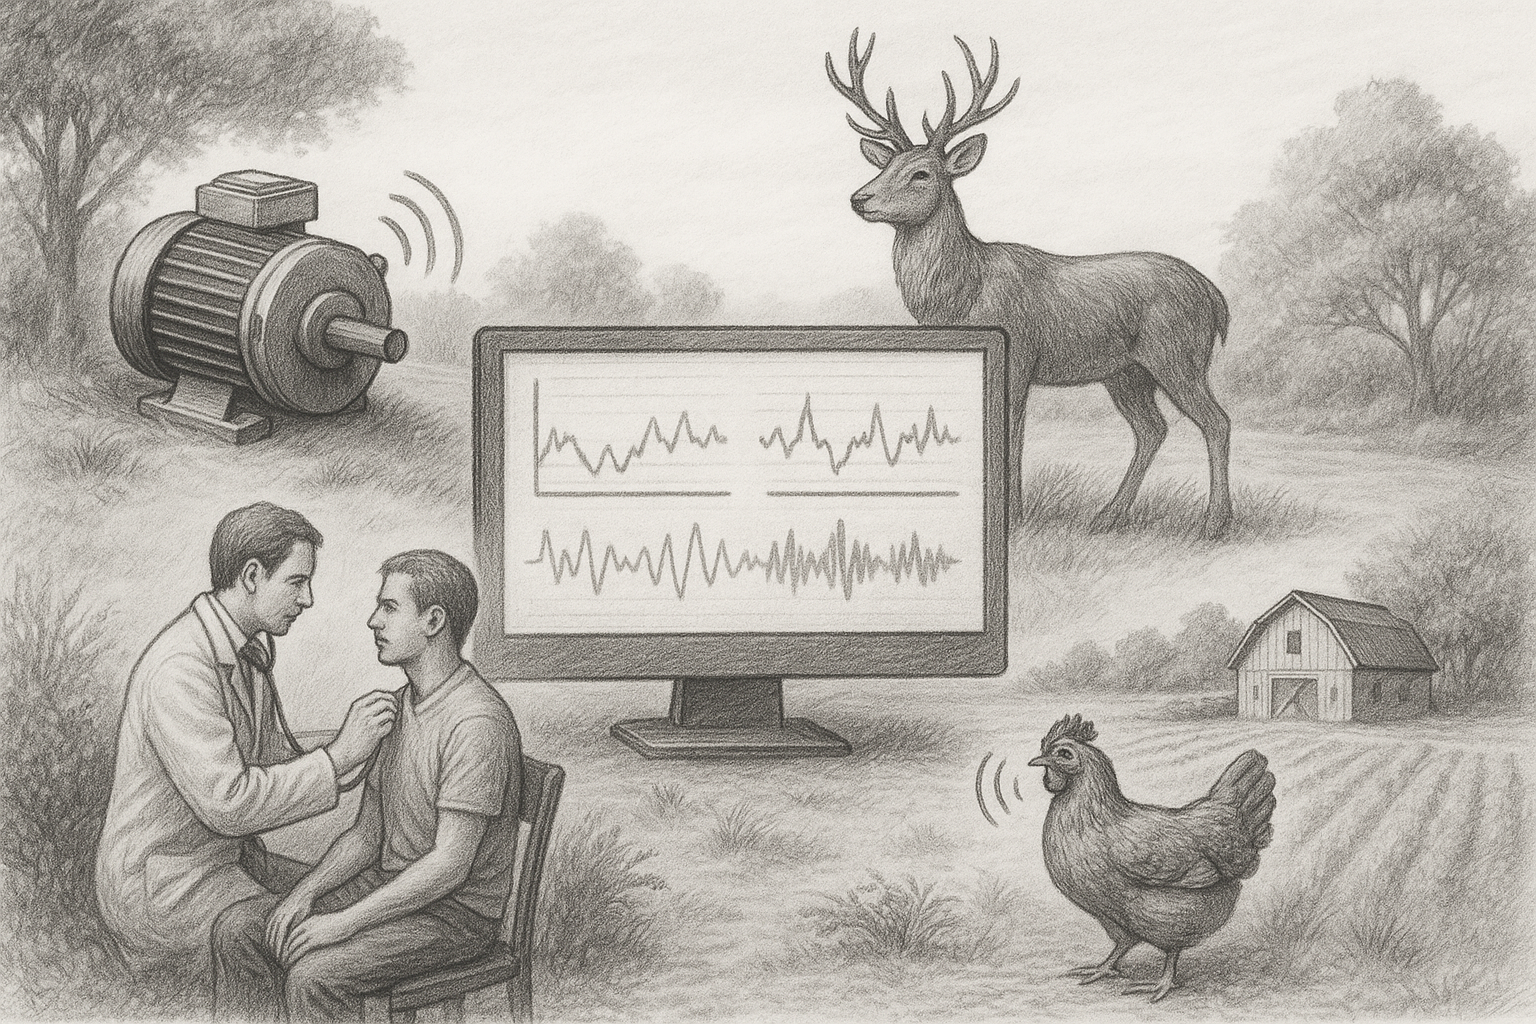
\includegraphics[width=0.75\linewidth]{Gambar/AudioBasedAnomalyDetection.png}
\caption{Konsep pendeteksian anomali berbasis audio}
\label{fig:audioanomaly}
\end{figure}

Setiap gambar yang disisipkan harus dirujuk dalam uraian naskah, baik sebelum maupun sesudah gambar ditampilkan. Selain itu, harus terdapat penjelasan yang memadai mengenai isi gambar, tujuan penyisipannya, serta keterkaitannya dengan pembahasan.

\subsection{Tabel}

Setiap tabel harus diberi nomor urut dan judul yang ditempatkan di atas tabel. Penomoran tabel mengikuti format nomor bab dan nomor urut tabel pada bab tersebut.

Sebagai contoh, karakteristik hubungan antara masukan dan keluaran suatu sistem dapat disajikan seperti pada Tabel~\ref{tab:hubungan}.

\begin{table}[!ht]
\centering
\caption{Hubungan antara masukan dan keluaran}
\label{tab:hubungan}
\begin{tabular}{|c|c|c|c|}
\hline
No. & Masukan 1 & Masukan 2 & Keluaran \\
\hline
1 & A & A & C \\
2 & A & B & D \\
3 & B & A & E \\
4 & B & B & F \\
\hline
\end{tabular}
\end{table}

Setiap tabel harus dirujuk dalam teks dan disertai penjelasan mengenai isi tabel, makna data yang disajikan, serta relevansinya terhadap pembahasan.

\subsection{Persamaan}

Persamaan matematis digunakan untuk menjelaskan hubungan antarvariabel, parameter, atau besaran yang digunakan dalam penelitian. Persamaan harus ditulis menggunakan lingkungan \texttt{equation} atau lingkungan lain yang sesuai dari paket \texttt{amsmath}.

Setiap persamaan yang akan dirujuk pada bagian lain naskah harus diberi label menggunakan perintah \verb|\label{}| sehingga nomor persamaan dapat dikelola secara otomatis dan konsisten.

Sebagai contoh, kode berikut:

\begin{tcolorbox}
\verb|\begin{equation}|
\verb|E = mc^2|
\verb|\label{eq:einstein}|
\verb|\end{equation}|
\end{tcolorbox}

akan menghasilkan Persamaan~(\ref{eq:einstein}).

\begin{equation}
E = mc^2
\label{eq:einstein}
\end{equation}

Setiap persamaan yang disajikan harus dirujuk dan dijelaskan dalam uraian naskah. Penjelasan tidak hanya mencakup tujuan penggunaan persamaan, tetapi juga arti setiap variabel, parameter, konstanta, dan satuan yang digunakan.

Sebagai contoh, apabila digunakan persamaan energi relativistik pada Persamaan~(\ref{eq:einstein}), maka penjelasan simbol-simbol yang digunakan dapat dituliskan sebagai berikut:

\begin{itemize}[topsep=0pt,itemsep=0pt,parsep=0pt,leftmargin=*]
\item $E$ adalah energi (Joule);
\item $m$ adalah massa benda (kg);
\item $c$ adalah kecepatan cahaya di ruang hampa ($\approx 3 \times 10^8$ m/s).
\end{itemize}

Penjelasan variabel dapat dituliskan dalam bentuk daftar, paragraf, maupun tabel sesuai dengan jumlah simbol yang digunakan. Untuk persamaan yang kompleks dan melibatkan banyak parameter, penggunaan tabel simbol lebih disarankan agar lebih mudah dibaca.

Beberapa ketentuan yang perlu diperhatikan dalam penulisan persamaan adalah sebagai berikut:

\begin{itemize}[topsep=0pt,itemsep=0pt,parsep=0pt,leftmargin=*]
\item Setiap persamaan harus dirujuk dalam teks sebelum atau sesudah persamaan ditampilkan.
\item Simbol, variabel, parameter, dan konstanta yang muncul pada persamaan harus dijelaskan ketika pertama kali digunakan.
\item Satuan setiap variabel atau parameter perlu dicantumkan apabila relevan.
\item Notasi yang digunakan harus konsisten di seluruh dokumen.
\item Simbol matematika ditulis menggunakan mode matematika (\textit{math mode}).
\item Persamaan yang diambil dari referensi lain harus mencantumkan sumber rujukan yang sesuai.
\end{itemize}

\section{Penulisan Kutipan Format IEEE}

Penggunaan kutipan dalam penulisan karya ilmiah bertujuan untuk mendukung argumentasi, memperkuat landasan teori, serta menunjukkan keterkaitan penelitian dengan karya ilmiah yang telah dipublikasikan sebelumnya. Meskipun demikian, isi naskah sebaiknya tetap didominasi oleh hasil analisis, pemikiran, dan kontribusi penulis, sehingga tidak menjadi kumpulan kutipan dari berbagai sumber.

Dalam penulisan tugas akhir, penggunaan kutipan perlu dilakukan secara proporsional dan relevan dengan konteks pembahasan. Penulis disarankan untuk lebih banyak menggunakan kutipan tidak langsung dibandingkan kutipan langsung agar alur penulisan tetap mengedepankan hasil sintesis dan pemahaman penulis terhadap sumber yang dirujuk. Setiap kutipan harus memberikan nilai tambah terhadap pembahasan dan mendukung pengembangan gagasan penelitian.

Berdasarkan cara penyajiannya, kutipan dapat dibedakan menjadi dua jenis sebagai berikut.

\begin{description}
    \item[Kutipan langsung] yaitu kutipan yang ditulis persis sama dengan sumber aslinya tanpa mengubah susunan kata, ejaan, maupun tanda baca. Kutipan langsung digunakan apabila redaksi asli sumber dianggap penting untuk dipertahankan.
    
    \item[Kutipan tidak langsung] yaitu kutipan yang memuat ide, konsep, atau hasil pemikiran dari sumber lain yang disampaikan kembali menggunakan kalimat dan gaya bahasa penulis sendiri tanpa mengubah makna aslinya.
\end{description}

Pada format sitasi \gls{ieee}, sumber rujukan dicantumkan menggunakan nomor referensi yang ditulis di dalam tanda kurung siku, misalnya \cite{IEEEReferenceGuide2023}. Nomor referensi tersebut merujuk pada entri yang bersesuaian dalam Daftar Pustaka.

\subsection{Kutipan Langsung}

Kutipan langsung adalah pengambilan teks dari sumber asli tanpa mengubah susunan kata, ejaan, maupun tanda baca yang digunakan oleh penulis sumber.

Kutipan langsung digunakan apabila penulis ingin mempertahankan redaksi asli karena dianggap penting, memiliki makna khusus, atau diperlukan untuk menjaga ketepatan informasi.

Beberapa ketentuan kutipan langsung adalah sebagai berikut:

\begin{itemize}[topsep=0pt,itemsep=0pt,parsep=0pt,leftmargin=*]
\item Teks yang dikutip harus sama dengan sumber aslinya.
\item Kutipan harus disertai sitasi yang sesuai.
\item Penggunaan kutipan langsung sebaiknya dibatasi dan hanya digunakan apabila benar-benar diperlukan.
\item Kutipan yang panjang dapat dipisahkan dari paragraf utama menggunakan format \textit{block quotation} sesuai dengan ketentuan yang berlaku.
\end{itemize}

Contoh:

\begin{quote}
"\gls{iot} merupakan paradigma yang memungkinkan objek fisik terhubung dan berkomunikasi melalui jaringan internet" \cite{Atzori2010}.
\end{quote}

\subsection{Kutipan Tidak Langsung}

Kutipan tidak langsung adalah penyampaian kembali gagasan, pendapat, atau hasil penelitian dari sumber lain dengan menggunakan kalimat dan gaya bahasa penulis sendiri tanpa mengubah makna aslinya.

Kutipan tidak langsung lebih disarankan dalam penulisan karya ilmiah karena menunjukkan pemahaman penulis terhadap sumber yang digunakan.

Contoh:
\glsreset{iot}
\begin{quote}
\gls{iot} memungkinkan berbagai perangkat fisik untuk saling
berkomunikasi dan bertukar informasi melalui jaringan internet
\cite{Atzori2010}.
\end{quote}

Meskipun menggunakan kalimat sendiri, sumber asli tetap wajib dicantumkan.

\subsection{Parafrasa}

Parafrasa merupakan bentuk khusus dari kutipan tidak langsung yang dilakukan dengan mengubah struktur kalimat, pilihan kata, atau cara penyampaian informasi tanpa mengubah makna yang terkandung pada sumber asli.

Parafrasa tidak berarti mengganti beberapa kata dengan sinonim. Penulis harus benar-benar menuliskan kembali gagasan sumber menggunakan susunan kalimat yang berbeda dan tetap mencantumkan sitasi yang sesuai.

\subsection{Pengutipan Data, Tabel, Gambar, dan Persamaan}

Data, tabel, gambar, diagram, grafik, maupun persamaan yang diambil atau diadaptasi dari sumber lain wajib mencantumkan sumber rujukan.

Contoh penulisan sumber pada gambar:

\begin{quote}
    Sumber: Diadaptasi dari \cite{contohReferensi}.
\end{quote}

Apabila gambar, tabel, atau persamaan digunakan tanpa perubahan, sumber asli harus disebutkan secara jelas. Jika dilakukan modifikasi, gunakan keterangan seperti "Diadaptasi dari" atau "Dimodifikasi dari".

\subsection{Hal-Hal yang Perlu Dihindari}

Dalam melakukan pengutipan, beberapa praktik berikut harus dihindari:

\begin{itemize}[topsep=0pt,itemsep=0pt,parsep=0pt,leftmargin=*]
\item Menggunakan ide, data, atau hasil penelitian orang lain tanpa mencantumkan sumber.
\item Menyalin teks secara langsung tanpa tanda kutip atau tanpa sitasi.
\item Melakukan parafrasa yang terlalu mirip dengan sumber asli.
\item Mengutip sumber sekunder tanpa alasan yang jelas apabila sumber primer dapat diakses.
\item Menggunakan sitasi yang tidak sesuai dengan sumber yang dirujuk.
\end{itemize}

Seluruh bentuk kutipan yang digunakan dalam tugas akhir harus mengikuti kaidah akademik, etika penulisan ilmiah, serta format sitasi \gls{ieee} yang berlaku pada dokumen ini.

\section{Penulisan Daftar Pustaka}

Daftar pustaka disusun menggunakan format sitasi \gls{ieee} sesuai dengan pedoman \gls{ieee} Citation Guidelines~\cite{IEEEReferenceGuide2023}. Seluruh sumber yang digunakan dalam penulisan tugas akhir harus dicantumkan dalam daftar pustaka dan dirujuk pada isi naskah.

Format sitasi \gls{ieee} menggunakan sistem sitasi numerik yang ditandai dengan nomor referensi di dalam tanda kurung siku, misalnya \cite{Simonovic2021}. Nomor referensi diberikan berdasarkan urutan kemunculan sumber pertama kali dalam naskah dan digunakan secara konsisten untuk sitasi berikutnya dari sumber yang sama \cite{IEEEReferenceGuide2023,IEEEEditorialStyleManual}. Oleh karena itu, sitasi dalam format IEEE dilakukan menggunakan nomor referensi dan tidak mengikuti konvensi sitasi berbasis catatan kaki yang menggunakan istilah seperti \textit{ibid.}, \textit{op. cit.}, atau \textit{loc. cit.}.

Bagi pengguna \LaTeX, referensi disarankan dikelola menggunakan \texttt{BibTeX} atau \texttt{BibLaTeX}. Seluruh metadata referensi disimpan pada berkas \texttt{referensi.bib}, kemudian dipanggil melalui perintah sitasi yang sesuai. Penggunaan sistem manajemen referensi ini bertujuan untuk menjaga konsistensi format sitasi dan mempermudah pengelolaan referensi.

Bagi pengguna Microsoft Word, referensi disarankan dikelola menggunakan perangkat lunak manajemen referensi seperti Zotero, Mendeley, EndNote, atau aplikasi sejenis yang mendukung format sitasi \gls{ieee}. Penggunaan perangkat lunak tersebut memudahkan proses penyisipan sitasi, penyusunan daftar pustaka secara otomatis, serta penyesuaian format sitasi apabila diperlukan.

Penulisan referensi secara manual sangat tidak disarankan karena berpotensi menimbulkan ketidakkonsistenan format dan kesalahan sitasi. Oleh karena itu, penggunaan perangkat lunak manajemen referensi dianjurkan untuk seluruh proses penyusunan tugas akhir.

\clearpage
\chapter{\MakeUppercase{Perancangan Sistem}}

Bab ini menjelaskan rancangan sistem yang diusulkan untuk menyelesaikan permasalahan yang telah dirumuskan pada bab sebelumnya. Perancangan dilakukan berdasarkan landasan teori, hasil studi pustaka, kebutuhan sistem, serta batasan masalah yang telah ditetapkan.

Tujuan utama bab ini adalah menjelaskan bagaimana solusi yang diusulkan akan diwujudkan sebelum dilakukan implementasi. Oleh karena itu, pembahasan pada bab ini harus berfokus pada rancangan sistem, bukan pada hasil implementasi atau hasil pengujian.

Secara umum, bab ini dapat memuat beberapa bagian berikut:

\begin{enumerate}[topsep=0pt,itemsep=0pt,parsep=0pt,leftmargin=*]
\item Gambaran umum sistem yang diusulkan.
\item Analisis kebutuhan sistem, baik kebutuhan fungsional maupun nonfungsional.
\item Arsitektur sistem secara keseluruhan.
\item Diagram blok sistem dan penjelasan fungsi setiap blok.
\item Diagram alir (\textit{flowchart}), \textit{state machine}, \textit{use case}, atau model lain yang sesuai.
\item Perancangan perangkat lunak, algoritma, metode, atau model yang digunakan.
\item Perancangan perangkat keras (jika ada), termasuk hubungan antar komponen dan antarmuka yang digunakan.
\item Perancangan basis data, format data, protokol komunikasi, atau struktur informasi yang digunakan.
\item Perancangan parameter, konfigurasi, dan skenario operasi sistem.
\end{enumerate}

Setiap rancangan yang dibuat harus disertai alasan pemilihannya. Apabila terdapat beberapa alternatif rancangan, jelaskan alasan mengapa rancangan tertentu dipilih untuk digunakan dalam penelitian.

Beberapa hal yang perlu diperhatikan dalam penyusunan Bab Perancangan Sistem adalah sebagai berikut:

\begin{itemize}[topsep=0pt,itemsep=0pt,parsep=0pt,leftmargin=*]
\item Fokus pada \textbf{apa yang akan dibuat dan bagaimana cara kerjanya}, bukan pada hasil implementasi.
\item Gunakan diagram, tabel, atau ilustrasi untuk memperjelas penjelasan sistem.
\item Setiap diagram harus dirujuk dan dijelaskan dalam uraian.
\item Jelaskan alur data, alur proses, masukan, keluaran, serta interaksi antar bagian sistem.
\item Pastikan seluruh rancangan mendukung pencapaian tujuan penelitian dan menjawab rumusan masalah.
\item Hindari pembahasan hasil pengujian, evaluasi, atau analisis performa pada bab ini karena pembahasan tersebut termasuk dalam bab implementasi dan pengujian.
\end{itemize}

Pada akhir bab, pembaca harus dapat memahami struktur sistem yang dirancang, prinsip kerja setiap bagian, serta alasan pemilihan metode, algoritma, maupun konfigurasi yang digunakan sebelum sistem diimplementasikan.

\clearpage
\chapter{\MakeUppercase{Hasil Pengujian dan Analisis}}

Bab ini menyajikan hasil implementasi, pengujian, serta analisis terhadap sistem yang telah dirancang. Tujuan pengujian adalah untuk memverifikasi bahwa sistem telah bekerja sesuai dengan spesifikasi, kebutuhan, dan tujuan penelitian yang telah ditetapkan.

Pada bab ini, hasil pengujian tidak hanya ditampilkan dalam bentuk data, tabel, grafik, atau gambar, tetapi juga harus dianalisis secara kritis untuk menjelaskan makna dari hasil yang diperoleh. Analisis yang dilakukan harus mampu menunjukkan tingkat keberhasilan sistem dalam menyelesaikan permasalahan yang dirumuskan pada penelitian.

Secara umum, isi bab ini dapat mencakup beberapa bagian berikut:

\begin{enumerate}[topsep=0pt,itemsep=0pt,parsep=0pt,leftmargin=*]
\item Deskripsi implementasi sistem yang telah direalisasikan berdasarkan rancangan pada bab sebelumnya.
\item Metode dan skenario pengujian yang digunakan.
\item Hasil pengujian setiap bagian atau fungsi sistem.
\item Hasil pengujian sistem secara keseluruhan.
\item Analisis terhadap hasil pengujian.
\item Perbandingan hasil yang diperoleh dengan target, spesifikasi, teori, penelitian terdahulu, atau standar yang digunakan sebagai acuan.
\item Identifikasi kelebihan, keterbatasan, dan faktor-faktor yang memengaruhi kinerja sistem.
\end{enumerate}

Dalam melakukan analisis, beberapa pertanyaan berikut sebaiknya dapat dijawab:

\begin{itemize}[topsep=0pt,itemsep=0pt,parsep=0pt,leftmargin=*]
\item Apakah sistem telah bekerja sesuai dengan rancangan?
\item Apakah tujuan penelitian telah tercapai?
\item Apakah hasil yang diperoleh sesuai dengan teori atau referensi yang digunakan?
\item Faktor apa saja yang memengaruhi hasil pengujian?
\item Apa kelebihan dan keterbatasan sistem yang dikembangkan?
\item Bagaimana hasil penelitian dibandingkan dengan metode, sistem, atau penelitian lain yang sejenis?
\end{itemize}

Setiap hasil pengujian yang disajikan harus didukung oleh data yang memadai. Data dapat disajikan dalam bentuk tabel, grafik, gambar, tangkapan layar, maupun bentuk lain yang sesuai. Seluruh data yang ditampilkan harus dirujuk dan dijelaskan dalam uraian sehingga pembaca dapat memahami konteks serta makna dari hasil yang diperoleh.

Hal-hal yang perlu diperhatikan dalam penyusunan bab ini adalah sebagai berikut:

\begin{itemize}[topsep=0pt,itemsep=0pt,parsep=0pt,leftmargin=*]
\item Jangan hanya menampilkan data tanpa analisis.
\item Analisis harus didasarkan pada fakta dan data yang diperoleh, bukan asumsi semata.
\item Setiap tabel, grafik, gambar, atau hasil pengujian harus dirujuk dan dijelaskan.
\item Hasil yang tidak sesuai harapan tetap harus dilaporkan dan dianalisis penyebabnya.
\item Analisis harus mengarah pada pembuktian bahwa tujuan penelitian telah atau belum tercapai.
\end{itemize}

Pada akhir bab, pembaca harus dapat memahami tingkat keberhasilan sistem yang dikembangkan, faktor-faktor yang memengaruhi kinerjanya, serta kontribusi hasil penelitian terhadap penyelesaian permasalahan yang diteliti.

\clearpage
\chapter{\MakeUppercase{Kesimpulan dan Saran}}

Bab ini berisi kesimpulan yang diperoleh dari hasil penelitian serta saran yang dapat digunakan sebagai masukan untuk pengembangan lebih lanjut. Kesimpulan dan saran harus disusun berdasarkan hasil analisis dan pembahasan yang telah dipaparkan pada bab sebelumnya.

\section{Kesimpulan}

Kesimpulan merupakan pernyataan ringkas yang merangkum hasil utama penelitian. Isi kesimpulan harus secara langsung menjawab rumusan masalah dan menunjukkan tingkat pencapaian tujuan penelitian yang telah ditetapkan.

Kesimpulan tidak diperkenankan memuat data baru, teori baru, atau pembahasan yang belum dijelaskan pada bab sebelumnya. Setiap kesimpulan harus didasarkan pada hasil pengujian, analisis, dan pembahasan yang telah dilakukan.

Dalam menyusun kesimpulan, beberapa hal berikut perlu diperhatikan:

\begin{itemize}[topsep=0pt,itemsep=0pt,parsep=0pt,leftmargin=*]
\item Kesimpulan harus menjawab seluruh rumusan masalah penelitian.
\item Kesimpulan harus menunjukkan apakah tujuan penelitian telah tercapai.
\item Kesimpulan disusun berdasarkan fakta dan hasil yang diperoleh selama penelitian.
\item Kesimpulan ditulis secara ringkas, jelas, dan tidak mengulang seluruh isi pembahasan.
\item Apabila memungkinkan, sertakan hasil atau capaian utama yang paling signifikan dari penelitian.
\end{itemize}

Kesimpulan dapat dituliskan dalam bentuk paragraf maupun butir-butir pernyataan sesuai dengan kebutuhan dan karakteristik penelitian.

\section{Saran}

Saran berisi rekomendasi yang diberikan berdasarkan pengalaman dan temuan selama pelaksanaan penelitian. Saran dapat ditujukan untuk pengembangan sistem, penyempurnaan metode, perluasan ruang lingkup penelitian, maupun penelitian lanjutan.

Saran harus bersifat konstruktif, realistis, dan relevan dengan hasil penelitian yang telah dilakukan. Saran tidak digunakan untuk memperbaiki kelemahan penulisan laporan, melainkan untuk memberikan arah pengembangan pada penelitian atau implementasi berikutnya.

Beberapa bentuk saran yang dapat diberikan antara lain:

\begin{itemize}[topsep=0pt,itemsep=0pt,parsep=0pt,leftmargin=*]
\item Pengembangan fitur atau fungsi yang belum diimplementasikan.
\item Peningkatan performa, akurasi, efisiensi, atau keandalan sistem.
\item Penggunaan metode, algoritma, atau pendekatan lain yang berpotensi memberikan hasil lebih baik.
\item Pengujian pada kondisi, lingkungan, atau skala yang lebih luas.
\item Pengembangan penelitian lanjutan untuk mengatasi keterbatasan yang masih ada.
\end{itemize}

Saran yang diberikan sebaiknya berkaitan langsung dengan keterbatasan, kendala, atau peluang pengembangan yang ditemukan selama penelitian berlangsung.

\clearpage
\addcontentsline{toc}{chapter}{\MakeUppercase{Daftar Pustaka}}
\printbibliography[title={\MakeUppercase{Daftar Pustaka}}]
\clearpage 
\chapter*{\MakeUppercase{Lampiran}}
\addcontentsline{toc}{chapter}{\MakeUppercase{Lampiran}}

Lampiran berisi materi pendukung yang digunakan dalam pelaksanaan atau penyusunan penelitian, tetapi tidak ditempatkan pada bagian utama naskah agar pembahasan tetap ringkas dan terfokus. Materi yang disajikan dalam lampiran harus tetap relevan dengan penelitian dan dapat membantu pembaca memahami, memverifikasi, atau mereproduksi hasil penelitian.

Dokumen yang dapat disertakan dalam lampiran antara lain kode sumber program, data mentah, tabel yang berukuran besar, hasil perhitungan rinci, instrumen penelitian, hasil pengujian tambahan, dokumentasi kegiatan, serta dokumen pendukung lainnya yang diperlukan. Materi yang disajikan dalam lampiran sebaiknya merupakan informasi yang penting untuk melengkapi penelitian, namun kurang sesuai apabila ditempatkan pada bab-bab utama Tugas Akhir karena dapat mengganggu alur pembahasan.

\clearpage
\end{document}
